As described in the previous chapter, the Turnover Box as very fundamental part of supply chain is the optimal experimental object to apply the blockchain technlogy. Before the development, this chapter will give an overview of the project design. It starts with the analysis of user requirements, then transfers the business model into conceptual model, in the end is the software and system design.


\section{Project description}
A Turnover Box system owner wants to implement an efficient, safe, automatically integrated comprehensive system to operate, control and manipulate the Boxes transactions with its cooperators.
\subsection{Product}
At end of the project, the Boxes operator, also as the owner will receive a blokchain-based system, on which all participants can do deal with Boxes. Only the owner can issue(add) new Boxes into the ledger as well as remove them.
\subsection{Roles}
In our scenario, there are mainly 4 roles:\\
\textbf{Box operator}: provides all types of the Boxes for delivering various products.

\textbf{Product Suppliers}: consume the Boxes as containers to transport various products.

\textbf{Distributors}: purchase the products from suppliers and then distribute them to different retailers. If received empty Boxes from retailers, the distributors should return those Boxes to the operator.

\textbf{Retailers}: order products from distributors and return the boxes either directly to operator or distributors. 

\bigskip
Figure 4.1 has clearly illustrate us how the participants in this network interact with each other and the flow of Boxes.
\begin{figure}[H]% use[!htb] to force the latex ignore the defaut
	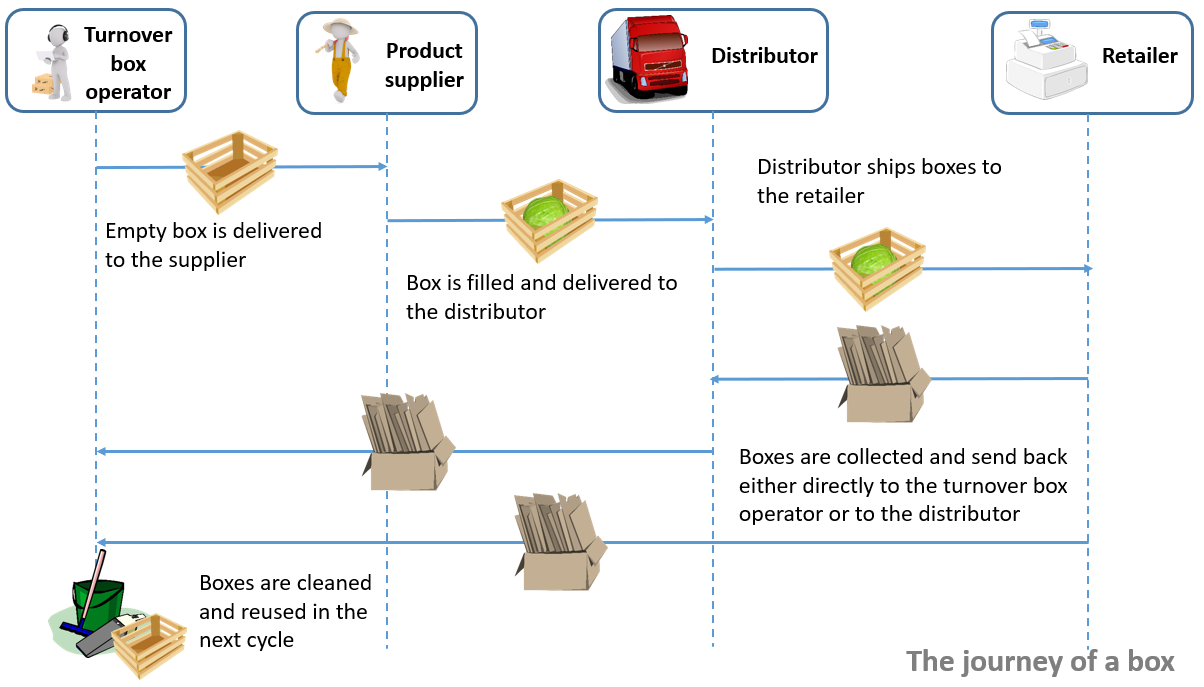
\includegraphics[width=0.9\textwidth]{charts/boxflow}
	\caption{The activity flow}
	\label{fig:label}
\end{figure}

\subsection{Pre- and post-conditions}
\subsubsection{Precondition}
\begin{itemize}
	\item There are two types of digital assets: Cash and Box.
	\item The number of Boxes should be positive.
	\item Participants' account should be positive.
	\item In the initial system, all participants' account should be zero.
	\item The Box has atomicity feature, which can not be partly treated.
	\item The Cash can be in any existing type of currency.
\end{itemize}
\subsubsection{Postcondition}
\begin{itemize}
	\item Ultimately, the income of the operator equals the outcomes of the suppliers and potential the rest of parties.
	\item Any parties who cause any damage to the Boxes should pay for the damage.
	\item There shouldn't exist any direct transaction between suppliers and retailers 
\end{itemize}

\section{Conceptual model}
A conceptual model is sufficiently comprehensive so that it can serve as a specification for developing software or a program, namely the simulation program. Setting up a conceptual model can help us
better understand the requirements, optimized the develop process, communicate with all parties involved and evaluate.
The conceptual model consists of a set of
components: the objectives, inputs, outputs, content, assumptions and simplifications of the model. 

According to the activity flow and the requirement, we can depict the conceptual model as Figure 4.2
\begin{figure}[!h]% use[!htb] to force the latex ignore the defaut
	\center
	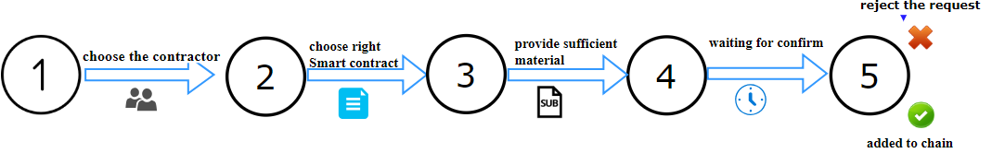
\includegraphics[width=1.1\textwidth]{charts/steps}
	\caption{conceptual model}
	\label{fig:label}
\end{figure}

In oder to have a better overview of the whole system, we draw the Figure 4.3. Participants can access the network through web or phone application.
\begin{figure}[!h]% use[!htb] to force the latex ignore the defaut
	\center
	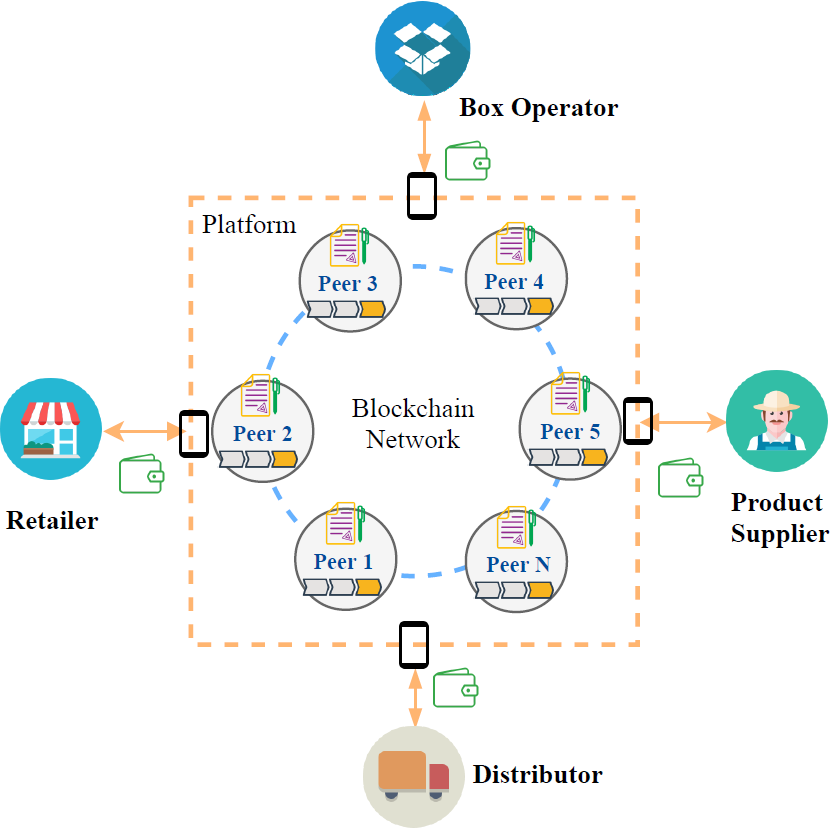
\includegraphics[width=0.9\textwidth]{charts/conceptual}
	\caption{overview graph}
	\label{fig:label}
\end{figure}

\section{Mapping into Smart Contract}

In the Figure 4.2, it demonstrates how the actual activities proceed.\\
We can also briefly conclude those mutual activities as following:
\begin{enumerate}
	\item Box operator \textbf{adds} new Boxes into the turnover box system.
	\item Product suppliers rent boxes from Box operator and \textbf{pay for the refuel fee}.
	\item Distributors purchase products from suppliers, and \textbf{pay for the pledge of the boxes}.
	\item Retailers place orders for products from distributors and \textbf{pay for the pledge}.
	\item Distributors and Box operator will \textbf{refund retailers the pledge} when retailers simultaneously restore the Boxes.
	\item Box operator \textbf{refunds distributors the pledge} when the Boxes are restored.
	\item Distributors \textbf{decide the box types} with Box operators. 
	\item Distributors require the supplier to use certain types of Boxes.	
\end{enumerate}
In sum, we want to translate the business logic into automatically executable program, that is called chain code or smart contract. Roughly now we could anticipate 5 main contracts.
\begin{itemize}
	\item \textbf{func addBox (boxinfo, ChaincodeStubInterface)}\\
		  The addBox function is the method turnover box Operators use to record of the new boxes coming into service. 
		  
	\item \textbf{func payforPledge(counterparties,Box.type, Box.num)}\\
	      The PayforFee method is the method actors use to pay for the Fee during the delivery.
	      
	\item \textbf{func damageCost(box.num, box.type)}\\
	      The damageCost method is designed to fine the party, which damages or loses the Boxes.
	      
	\item \textbf{func refund(counterparty, box.type, box.num)}\\
	      The Refund method is the method actors use to refund the Fee during the delivery. This contract should be similar to the payforFee method.
	      
	\item \textbf{func deposit(party, num)}\\
	      Recharge method is extremely crucial method in the supply chain, since the Hyperledger Fabric, and Corda has no token and wallet, so we devise Recharge method as a prepay contract, 
	      All the actors can only deposit at the turnover box operators. After recharging the deposit
	      can be written as digital assets store in the Blockchain
\end{itemize}


